\documentclass{acm_proc_article-sp}

\usepackage{natbib}
\usepackage{url}

\makeatletter
\def\@copyrightspace{\relax}
\makeatother

\begin{document}

\title{SMS Immunization Manager (SIM)}

\numberofauthors{4} 
\author{
       % \alignauthor
       Jenny Kang, Isaac Reynolds, Jackson Roberts, Nicholas Shahan\\
              \affaddr{University of Washington}\\
              \affaddr{Seattle, WA, USA}\\
              \email{jskang, isaacr, jcwr, nshahan@uw.edu}
}

\maketitle
\begin{abstract}
There is a great need for timely and accurate reports in order to facilitate the efficient distribution of vaccines across health centers within a country. The SMS Immunization Manager (SIM) is a system designed to improve the efficiency of vaccine cold chains. SIM provides health workers with an easier and more reliable way of reporting vaccine stock levels and the status of crucial equipment, in order to replace the existing paper-based reporting system. SIM fulfills two main functionalities. First, it receives messages and acts on behalf of them though the use of different programmable modules. Second it provides a web-based user interface to allow for administration of users and moderation of the effects generated by the incoming messages. While this project was built with Laos specific requirements in mind, SIM was designed to be easily customized and scaled in order to be deployed for use in aiding the management of vaccine cold chains in other countries as well.  
\end{abstract}

\section{Introduction}
Coordinated, national efforts (supported by organizations such as UNICEF, WHO, and hundreds of NGOs and universities) to distribute vaccines in developing countries have proven to be among ``the most successful and cost-effective health interventions'' in human history. These programs currently prevent between two and million deaths per year. However, even as recently as in 2008, nearly 17\% of the 8.8 million deaths in infants and young children were from diseases that could have been prevented by vaccination \cite{who:campaign_essentials}. 

Improving the effectiveness of vaccine distribution programs requires improving distribution networks in existing deployment programs as well as instituting new programs in poorly-covered countries. Our project focuses on the former by augmenting an existing deployment system in Laos (their distribution process is discussed below). However, many of the processes and motivations described below are similar for other countries as well, so our project can be useful for countries other than Laos.

The current system in Laos distributes vaccines down a hierarchy on a monthly cycle. Each step lower in the hierarchy contains smaller facilities with progressively lower capacity, fewer staff, less frequent restocking, poorer roads, and less reliable equipment, power, cell service, and Internet (if available at all). Each vaccine must be kept refrigerated at a specific temperature to avoid spoiling, so this chain of facilities through which vaccines pass is called the ``cold chain''.

Facilities at the lowest tier of the hierarchy operate on roughly a monthly schedule (sometimes less often for particularly remote stations). Every month, workers at the next higher tier fill a small truck with ice chests full of vaccine and then spend about two weeks driving a loop through outposts on the lowest tier. At each facility, the workers resupply vaccine stock (once at an outpost, the vaccines are kept in propane- or electricity-powered refrigerators), collect information about the previous month's demand and vaccine spoilage, and perform any necessary repairs. The information they gather is used to plan the next deliveries. 

Most vaccinations are done by the Community Health Workers at these smallest facilities. People travel for hours by foot to get their children vaccinated, often forgoing other vital tasks. They either travel directly to the outpost, or to an event in some other community that a CHW has scheduled in advance (sometimes CHWs pack bags with vaccines and walk around neighboring communities to do vaccinations). 

Being vaccinated is a large time investment for most individuals, so it's important that there's enough unspoiled stock to satisfy the demand for vaccinations. Individuals who travel for hours only to find that there is no vaccine left are less likely to return again, and they may recommend the same to others. 

Furthermore, running out of stock is a real concern. High demand, low supply, a broken or failing fridge, interruptions in power supply, or temperatures high or low enough to overwhelm fridges can all cause unexpected stock outages. Giving higher-level distributors timely access to reliable information can prevent stock outages as well as mitigate the effects of outages that do occur. 

Unfortunately, the current data collection schedule means that each facility is resupplied based on data that is four to eight weeks old (imagine: a facility is resupplied on June 15th based on data collected on May 15th about the reporting period starting April 15th). Any improvement in this aspect of distribution requires an alternate form of reporting. 

\subsection{SMS-Based Reporting}

We present SMS Immunization Manager (SIM), a framework that allows CHWs to report information about the vaccine cold chain (such as fridge temperature and condition) quickly by SMS. SIM's main features include 

\begin{itemize}
\item Robust SMS-based operations that correctly handle even poorly-formatted messages through careful design of message formats. The included operations were inspired by a current need in Laos.
\item A moderation web application for administrators to review the system's operation.
\item A simple and well-documented design that enables one or two developers to deploy a complete system in only several weeks.
\end{itemize}

The system will be deployed in Laos in mid-2014, replacing an existing prototype \cite{unicefstories}, but it is useful for any cold chain reporting system and could easily be adapted for new deployments. A diagram describing how SIM interacts with surrounding systems is shown below.

% figure* clears both columns, and figure clears one.
% Download the image from source as PDF.
% If the image is too large or small, the best solution is to resize the source you downloaded and then re-downloaded. Continue until it's the correct size.
\begin{figure*}
\centering
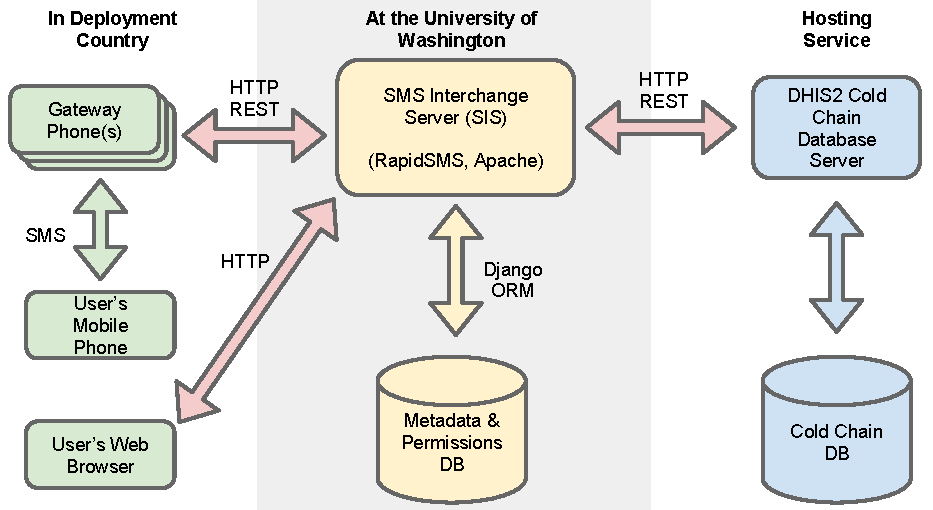
\epsfig{file=sim-broad-diagram.pdf}
\caption{SIM's relationship with other systems.}
\end{figure*}

SIM communicates exclusively via HTTP, which means it can be deployed on any web host. In order for CHWs to communicate with SIM via SMS, a ``gateway device'' must be deployed on the CHW's cellular network or a connected cellular network. The gateway device may be as simple as a midrange Android phone (the system was originally implemented using EnvayaSMS running on such a phone), or it may be as complex as a high-load dedicated gateway provided by the cellular provider. 

Although SIM was built to handle poorly-formatted SMS messages typed by hand by people with little access to training, there is no requirement that messages are hand-typed. The messages could just as easily be created by a simple application running on an embedded controller---for example, the FoneAstra system could automate data reporting by sending properly-formed SMS messages to SIM \cite{foneastra}.

The choice of where and when to use SMS and HTTP protocols was made carefully. The majority of users, especially CHWs reporting cold chain data, are without reliable access to Internet and power. This limits HTTP's usefulness. However, cell coverage in developing countries is good; recent estimates say that roughly five billion people in developing countries have access to a cell phone \cite{worldbank:mobileaccess}. SIM only requires several minutes of coverage per report and expects one or two reports per month, which we expect to be manageable.

However, SIM requires the gateway to have Internet access so that it may relay messages between SMS users and the SIM server. It also requires that moderators have Internet access. This allows SIM to provide a powerful, usable, bug-free moderation interface to review the system's operation.

In order to prevent malicious or accidental misuse, SIM only allows access from registered users (SMS users and moderators), each of whom is assigned one of several ``roles'' (with associated permissions). Among other things, privileged SMS users may register new users via SMS (for example, the facility manager would be able to register any other workers), and privileged moderators can access special tools for administering the Django and RapidSMS architectures on which SIM is based. This user information, which also includes each user's preferred language, is kept in a database managed by SIM.

However, SIM does not attempt to store any more cold chain information than necessary (typically only the facility hierarchy). Instead, SIM is intended to pass all of this data to a complete remote cold chain information/equipment management system such as DHIS2. That remote database is the permanent repository for cold chain data because it provides powerful querying and visualization tools (SIM does not, and is not intended to).

CHWs interact with SIM by sending structured SMS messages. Common use cases in Laos include

\begin{itemize}
\item A CHW periodically (monthly or more) sends one SMS message including both (a) their facility's current stock of each vaccine and (b) the number of times each of their fridges dipped below or rose above ideal temperature during the reporting period. Fridge data in Laos is recorded automatically by a Fridge-tag \textsuperscript{\textregistered} \cite{fridgetag}. If the CHW's message is too poorly-formatted to interpret, within several minutes a useful error message is returned (otherwise, a ``thank you'' message is returned). 
\item A facility unexpectedly runs out of stock of a particular vaccine, so a worker at the facility sends, as soon as possible, an SMS message identifying the vaccine. The stock outage is brought to the attention of the moderator the next time they log in so the outage can be handled rapidly. The same process can be used if any equipment fails.
\item It is a fact of life that workers come and go, change facilities, and change SIM cards. Privileged SMS users can register a new data reporter with a name, phone number, and associated facility by sending a single SMS message. Any worker can also change their preferred language at any time and see all SMS responses in that language.
\end{itemize}

Moderators interact with SIM by using a web application. Common use cases in Laos include

\begin{itemize}
\item Any incoming SMS messages that failed (for syntax or permissions reasons) are brought to the attention of a moderator. The notification persists in the moderation application until the moderator explicitly views and dismisses the source of the error. Errors are viewed in the context that sender's other messages, which allows moderators to track individuals and make informed decisions about how to handle a particular user's situation
.\item When viewing an SMS message with an error, a moderator can edit the message and resend it (internally, without incurring SMS charges) with any explicit permissions level. This gives moderators the power to quickly correct messages that the system cannot understand but a human can.
\item Moderators can view per-message logs of every side effect the message produced and each operation the system applied to the message (including parsing, verifying permissions, filtering for spam, etc.). This allows moderators to quickly identify bugs in the system and provide accurate and useful bug reports to developers.
\end{itemize}

We believe that SIM is the first step toward a powerful reusable framework for simple-to-deploy and simple-to-use SMS reporting systems.

\section{Related Work}

Using SMS operations to resolve failures in cold chain reporting is not a new idea. There are many projects, including research projects, commercial technologies, development frameworks, and extensions of existing software that address a similar problem. Many of these products have been deployed, and many have had more time to collect requirements and features than SIM has had.

However, SIM has several fundamental differences from these packages that make it a better solution if a programmer is available for several weeks to construct the SMS operations.

One solution is to use ``DHIS2 Mobile SMS Commands''. DHIS2 is a widely-used, powerful, open-source cold chain information/equipment manager. Because the SMS commands are supported on the same platform as the permanent data store, the integration between them is perfect. For example, the most up-to-date information about facilities and data is always available and any DHIS2 form can be turned into an SMS command. Furthermore, this module is meant to be used by non-technical staff, so new custom SMS operations with syntax and behavior can be configured through a web application. There are many behaviors, including scheduled notifications, data updating, listserves, and data queries. It is a powerful and complete solution \cite{dhis2:smsref, dhis2:smsoverview}.

However, the DHIS2 system has several limitations that SIM does not. First, it requires that DHIS2 is the deployment's permanent data store (however, the country may already be using a different solution or would prefer something a different one). Second, configuring SMS syntaxes in a web interface (SIM defines this in code instead) as DHIS2 does produces syntaxes that require careful delimiting with special characters (including the `+' and space characters), which is more difficult for data reporters to use. Third, there is little capacity to define custom actions or behaviors separate from what DHIS2 has implemented, so some behaviors may be impossible to obtain and others may be more complex than necessary. Finally, and perhaps most importantly, there is no way for moderators to see detailed logs of incoming SMS messages, especially ones that were rejected. This makes it difficult to diagnose common errors (fixing the syntax to reduce errors is be difficult as well) and identify particular people or facilities that require training \cite{dhis2:smsref, dhis2:smsoverview}.

In order to address syntax problems, DHIS2 publishes a Java Micro Edition (J2ME) application that can be installed on cell phones from many vendors (although DHIS2 recommends that the country buy and distribute a common device to provide better support and reliability). The application presents a user interface with input fields for the user to fill in, and then the phone produces a well-formatted SMS message to send to the server \cite{dhis2:smsoverview, dhis2:j2me}. This is an effective solution, but requires the country purchase and distribute dozens of hundreds of phones and to invest in both creating, deploying, supporting, and updating an application installed on those devices.

Another solution more similar to SIM is RapidSMS. In fact, SIM is based on RapidSMS, but with several key changes (which are discussed later, but whose motivations are discussed here). RapidSMS allows syntax and behavior to be described in code, just as SIM does. It's also written in the powerful Python language and based on a widely-used rapid web development framework called Django. This makes RapidSMS easy to customize and deploy. However, RapidSMS (and SIM by extension) requires programmers in order to implement new behaviors and syntaxes while other solutions can generate these based on configuration by non-technical users through a web interface. The RapidSMS XForms library attempts to mitigate this by allowing syntaxes, at least, to be defined in a similar way to DHIS2 (though with similar limitations), but not behaviors \cite{rapidsms:overview, rapidsms:xforms}.

SIM is a framework based on RapidSMS (and this release represents an implementation of a reporting system for Laos using the SIM framework). While offering the same benefits as RapidSMS does (ease of deployment and ease of customizing syntaxes and behaviors), SIM also provides two further benefits: 

\begin{itemize}
\item Looser coupling between operation syntax and behavior. RapidSMS suggests implementing policy decisions about behaviors (including updating remote databases, checking permissions, and more) in the same place as the syntax is defined. This means that changing a policy about behavior can require modifying code in many locations across many files. SIM, however, uses the observer design pattern to centralize and separate policy decisions so they can be modified or replaced easily in a single location in the codebase without risking interfering with other behaviors.
\item A powerful and easily-integrated moderation interface. Any module that interacts with a message registers at least one ``effect'' in the database. The moderation interface merely displays these effects to the moderators. This both encourages developers to keep consistent, rich, and useful logs (in the form of these ``effects''), the benefits of which are well-known, and produces a minimal coupling between implementing new syntaxes/behaviors and integrating them into the moderation interface.
\end{itemize}

RapidSMS was the only framework that offered the flexibility that our requirements dictated, and even then it was not flexible or featureful enough to satisfy our requirements (especially because RapidSMS cannot allow multiple independent operations per SMS message, which we require). For that reason, we chose to implement a new framework. SIM has many advantages---it's easy to deploy, customize, and moderate as well as free to use and well-documented---that no single other framework provides.

\section{Approach}

\section{Implementation}

\section{Evaluation}

\section{Conclusion and Future Work}

\section{Acknowledgements}

We would like to thank Profs. Richard Anderson and Ruth Anderson for organizing CSE 481, providing us with a project to build, gathering requirements for our project, and connecting us with users and others who could provide feedback on SIM. We would also like to thank Trevor Perrier and Fahad Pervaiz for gathering requirements in Laos, implementing and deploying a valuable prototype, and taking over the project after CSE 481. We would also like to thank Ron Pankiewicz from VillageReach, who met with us twice to help define SIM's requirements and to provide feedback; Rajit Dhiman, who helped define requirements; and Lee, the IT administrator in for the Laos health ministry, who provided valuable feedback.

\bibliographystyle{abbrv}
\bibliography{report}  
\balancecolumns

\appendix
Many additional materials are available in our public code repository, on GitHub as ``ireynolds/sms-immunization-manager''. A comprehensive documentation site, which can be built and previewed using the nanoc static site generator, is available in the repository in the website/ directory.

\begin{figure*}
\centering
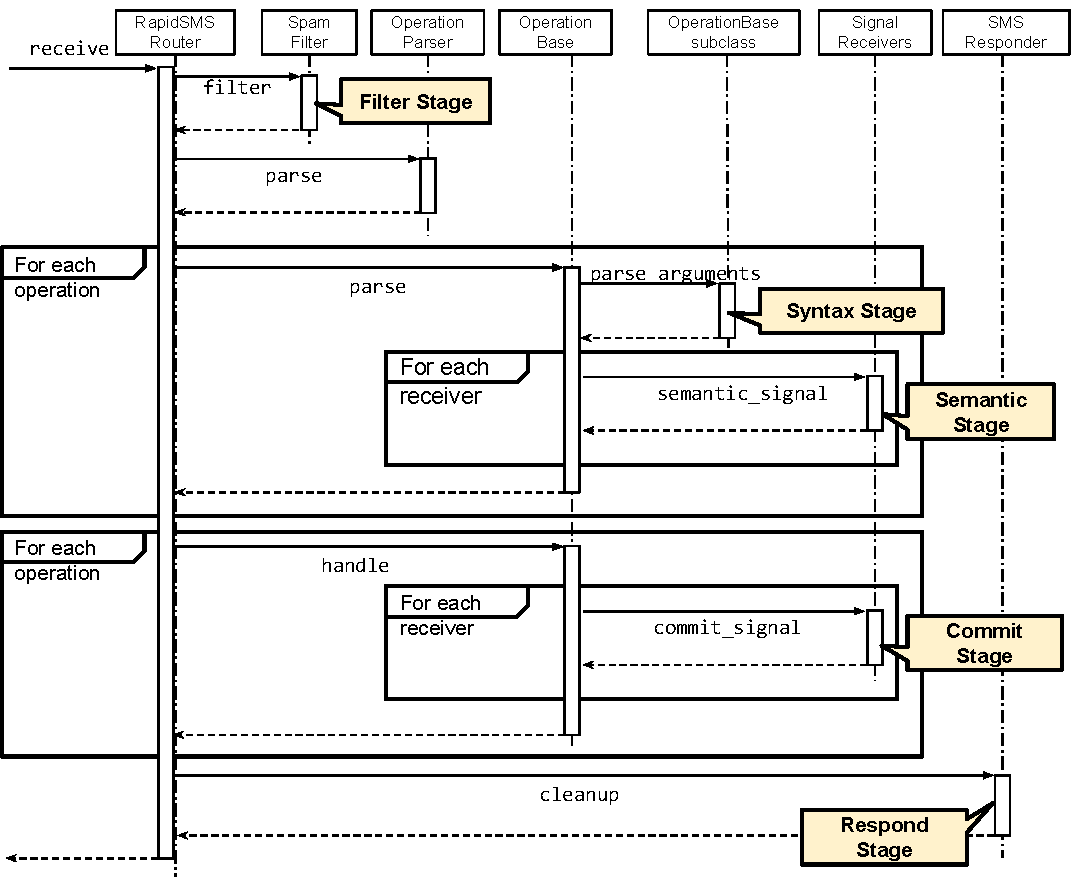
\epsfig{file=appendices/adapter.pdf}
\caption{RapidSMS/SIM Adapter Sequence Diagram}
\end{figure*}

\end{document}
